\section{System Design}
In this section we describe key aspects of our system design which increase the throughput of inter node communication and underline framework implementation details. First of all it is worth to note that even with one TCP connection, it is possible to saturate the network link usage, if the sending and receiving processes send and receive byte arrays without any delay even with 256 bytes array messages. However serializing java object messages to byte arrays and deserializing byte arrays back to java objects take considerable amount of time. Hence the key aspect of  improving the system performance is to reduce this message conversion delay. We use multitasking and bulk message serializing to solve this problem.

In this design, we use thread pools both at client side and server side to process messages while sharing a single TCP connection. Firstly both thread pools access underline connection resource only to send and receive byte arrays making message serialization and deserialization process parallel. Secondly it buffers the messages and serializes together.  This makes sure it produces large enough binary messages to fully utilize the underlying network and minimize the number of runtime objects created for message conversion. Figure \ref{interprocess} shows the design involved in sending a message from one process to another. 

Let's assume client side process requires to send a set of messages to server side process. In order to send these messages, first the client process threads send these messages to its \textit{ElementContainer}. \textit{ElementContainer} holds all the streams (this is an abstraction of a link in the process graph) to which these messages need to be send and it pushes each message to all the streams. Stream decides the target node and buffers messages for a configured amount of size. Then it passes the buffered  message list along the target node details to \textit{ConnectionManager} which holds \textit{ClientConnection}s for each node. \textit{ConnectionManager} serializes the message list and sends the byte array to correct \textit{ClientConnection} using the target node. \textit{ClientConnection} uses the \textit{DataOutput} which wraps the TCP connection to send message to server side. 

At the server side there is a set of \textit{ServerTask}s which reads receiving messages from a pool of \textit{DataInput} streams available in the \textit{ServerConnection} (we register these connections at the connections creating time) and send them to appropriate processes. First a server task acquires a \textit{DataInput} stream and reads the binary message and release it. Then it deserializes the binary message using the sending process id to identify the event type.  After that it passes this message to the \textit{WorkerContainer} which holds all processes. Finally \textit{WorkerContainer} dispatches this message to correct process using receiving process id. Message ordering happens at the process level if required. 

\begin{figure}[!t]
        \centering
        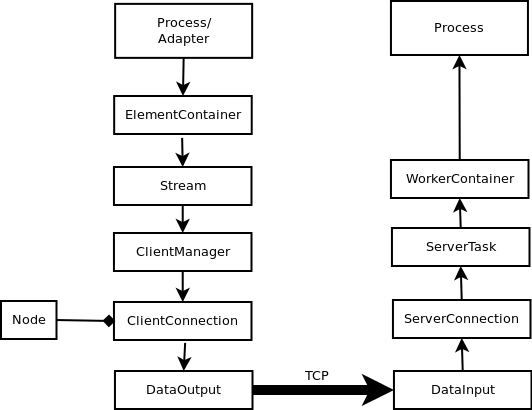
\includegraphics[width=3.0in]{interprocess.png}
        \caption{Communication between two Process}
        \label{interprocess}
\end{figure}

\subsection{Application message processing}
We use \textit{DataOutputStream} with \textit{ByteArrayOutputStream} to serialize application messages to binary format as batches and \textit{DataInputStream} with \textit{ByteArrayInputStream} to deserialize from the binary format. First four bytes of the binary format is used to specify the number of messages in the batch.  Deserializer use this information to read the exact amount of messages from the binary message. As mentioned earlier, we minimize these object creation by processing messages together. We also experimented with Kryo \cite{kryo}. Kryo provides an efficient binary format in terms of number of bytes used but that causes less throughput compared to above mechanism. 

\subsection{Binary Message Communication}
Once the application messages are converted to binary format, binary messages need to be send to the server side. At the client side we use \textit{DataOutput} to write the message length with the message and at the server side, we use \textit{DataInput} to read messages according to the length. \textit{DataOutput} and \textit{DataInpu}t interfaces requires \textit{OutputStream} and \textit{InputStream} objects to write and read data. We implement those interfaces with java non blocking I/O API as given bellow. This implementation allow as to re use the underline \textit{ByteBuffer} objects. 

\begin{figure}[!t]
        \centering
        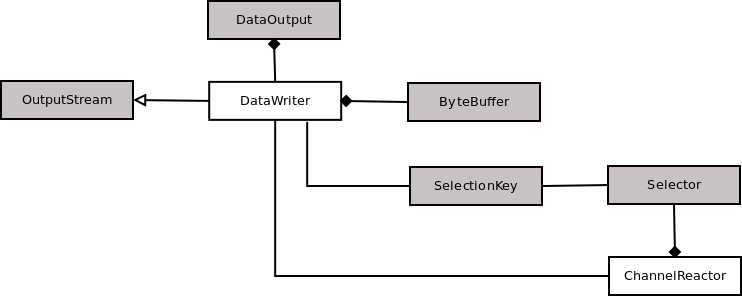
\includegraphics[width=3.0in]{client.png}
        \caption{OutputStream interface implementation with java blocking API}
        \label{client}
\end{figure}
\begin{figure}[!t]
        \centering
        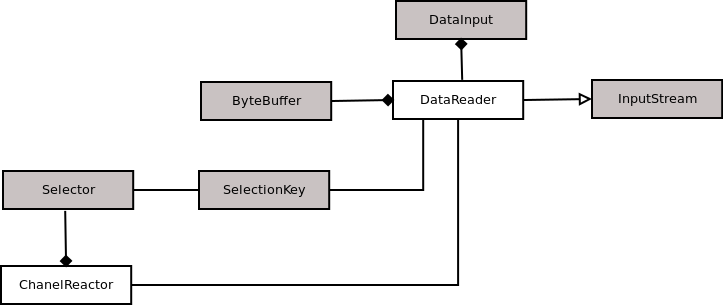
\includegraphics[width=3.0in]{server.png}
        \caption{InputStream interface implementation with java blocking API}
        \label{server}
\end{figure}

At client side (Figure \ref{client}), \textit{DataWriter} (implementation of  OutputStream) contains a \textit{ByteBuffer}. When a higher layer method writes data to \textit{DataOuput}, \textit{DataWriter} put those bytes to its \textit{ByteBuffer}. When a selection event occurs, \textit{Datawriter} writes its \textit{ByteBuffer} to underline \textit{SocketChannel}. At server side (Figure \ref{server}), \textit{DataReader} contains a \textit{ByteBuffer} similar to client side. When a selection event occurs \textit{DataReader} input bytes from the \textit{SocketChannel} to its \textit{ByteBuffer}. When a \textit{ServerTask} reads data through \textit{DataInput}, it reads data from the \textit{ByteBuffer} and passes to higher layer. 

\subsection{Load balancing}
Load balancing is the primary means of achieving data parallelism in stream processing. Each stage of the processing graph can be deployed into several nodes and can balance the load to next stage. In our framework load balancing happens at the \textit{Stream} level specific to the stream. \textit{KeyStream} balances the load by distributing keys among the nodes. \textit{RandomStream} balance messages randomly among next level of nodes. As mentioned above, buffering of the messages happens at the \textit{Stream} level. Further users can plug any custom stream with any specific partitioning function as well.

\subsection{Fault tolerance}
Fault tolerance is the ability of a system to operate with the presence of failures. These failures can be node failures or network failures and requirements to operate are depend on the system. In our framework, we provide fault resilient or ability to balance the load for existing nodes in the presence of node failures. If a receiving node fails then there will be a failure at the TCP connection and we close such connections and remove nodes from the \textit{Streams} (Stream objects hold the receiving node details). This prevents further routing messages to failure nodes.
